\renewcommand{\thesubsection}{\textcolor{red}{\Roman{section}.\arabic{subsection}}}
\renewcommand{\thesubsubsection}{\textcolor{red}{\Roman{section}.\arabic{subsection}.\alph{subsubsection}}}

\setcounter{section}{0}
\setcounter{document}{0}
\sndEnTeteActUn

\begin{center}
\begin{mdframed}[style=titr, leftmargin=60pt, rightmargin=60pt, innertopmargin=7pt, innerbottommargin=7pt, innerrightmargin=8pt, innerleftmargin=8pt]

\begin{center}
\large{\textbf{Activité 1 : Composition d'un mélange eau-huile}}
\end{center}

\end{mdframed}
\end{center}
\begin{Large}{\textbf{Q : Quelle est la proportion volumique et massique de l'huile et de l'eau présent dans l'éprouvette graduée sur le bureau du professeur ?}} \end{Large} 
\begin{mdframed}[style=autreexo]
\textbf{\bsc{Consignes :}}
\begin{itemize}
    \item Lever la main si vous souhaitez vous déplacer,
    \item Lever la main si vous souhaitez un indice,
    \item Vous pouvez travailler en binôme \textbf{\underline{uniquement}} avec votre voisin de table,
    \item Vous pouvez rendre le travail à la fin de l'heure si vous améliorer votre note d'interrogation.
   
\end{itemize}
\end{mdframed}

\begin{doc}{Lecture d'un volume sur la verrerie}

\begin{wrapfigure}{r}{0.3\textwidth}
\vspace{-2cm}
    \centering
      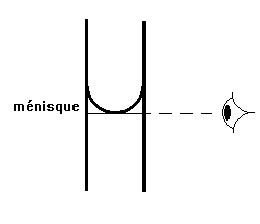
\includegraphics[width=0.27\textwidth]{Images/Lecture_Verrerie.png}
  \end{wrapfigure}
  Lorsqu'on verse un liquide dans une pièce de verrerie (éprouvette, tube à essai, etc), l se forme un ménisque qui va perturber la mesure du volume sur cette verrerie. Pour lire le volume occupé par un liquide, il faut positionner son \oe il sur le bas du ménisque.%En 1775, Antoine Lavoisier réalise une expérience qui lui permet de déterminer la composition de l’air.
%Son expérience est résumée dans la vidéo suivante : \url{https://ladigitale.dev/digiplay/#/v/6305f2f7b8fd4}.\\
%D’après Lavoisier, l’air est constitué de deux gaz : le dioxygène et le diazote. Le volume du gaz initialement
%présent dans la cloche est de 0,80 L d’air. À la fin de l’expérience, le volume du gaz qui n’a pas réagi avec le
%mercure (c’est-à-dire le diazote) est de 0,66 L.}
\end{doc}

\begin{doc}{Proportion volumique ou massique d’une espèce dans un mélange}
Pour décrire la composition d’un mélange, on indique la proportion (ou le pourcentage) de chaque espèce chimique constituant le mélange. On peut choisir d’utiliser la proportion massique notée $x_m$, ou la proportion volumique notée $x_V$ :
\begin{align*}
    x_m &= \frac{m_{\text{espèce}}}{m_{\text{totale}}} & x_V & = \frac{V_{\text{espèce}}}{V_{\text{totale}}}\\
\end{align*}
Ces deux grandeurs s'expriment en général en \%.
\end{doc}

\begin{doc}{Données utiles}
La masse volumique de l'huile est :
\begin{equation*}
    \rho_{huile} = 0,92 \text{~g.cm$^{-3}$}
    \end{equation*}
\end{doc}
